\documentclass{article}
% Change "article" to "report" to get rid of page number on title page
\usepackage{amsmath,amsfonts,amsthm,amssymb}
\usepackage{setspace}
\usepackage{Tabbing}
\usepackage{fancyhdr}
\usepackage{lastpage}
\usepackage{extramarks}
\usepackage{chngpage}
\usepackage{gensymb}
\usepackage{soul,color}
\usepackage{graphicx,float,wrapfig}
\usepackage{listings}


% In case you need to adjust margins:
\topmargin=-0.45in      %
\evensidemargin=0in     %
\oddsidemargin=0in      %
\textwidth=6.5in        %
\textheight=9.0in       %
\headsep=0.25in         %

% Homework Specific Information
\newcommand{\hmwkTitle}{Revised Project\ Proposal}
\newcommand{\hmwkDueDate}{Autumn\ 2011}
\newcommand{\hmwkClass}{CSE\ 634}
\newcommand{\hmwkClassTime}{9:30}
\newcommand{\hmwkClassInstructor}{Prof. James W. Davis}
\newcommand{\hmwkAuthorName}{Michael Schoenberg, Andrew D. Yates, Daniya Zamalieva}


% Setup the header and footer
\pagestyle{fancy}                                                       %
\lhead{\hmwkAuthorName\\}                                                 %
\chead{\hmwkClass\ (\hmwkClassInstructor\, \hmwkClassTime): \hmwkTitle}  %
\rhead{\firstxmark}                                                     %
\lfoot{\lastxmark}                                                      %
\cfoot{}                                                                %
\rfoot{Page\ \thepage\ of\ \pageref{LastPage}}                          %
\renewcommand\headrulewidth{0.4pt}                                      %
\renewcommand\footrulewidth{0.4pt}                                      %

% This is used to trace down (pin point) problems
% in latexing a document:
%\tracingall

%%%%%%%%%%%%%%%%%%%%%%%%%%%%%%%%%%%%%%%%%%%%%%%%%%%%%%%%%%%%%
% Some tools
\newcommand{\enterProblemHeader}[1]{\nobreak\extramarks{#1}{#1 continued on next page\ldots}\nobreak%
                                    \nobreak\extramarks{#1 (continued)}{#1 continued on next page\ldots}\nobreak}%
\newcommand{\exitProblemHeader}[1]{\nobreak\extramarks{#1 (continued)}{#1 continued on next page\ldots}\nobreak%
                                   \nobreak\extramarks{#1}{}\nobreak}%

\newlength{\labelLength}
\newcommand{\labelAnswer}[2]
  {\settowidth{\labelLength}{#1}%
   \addtolength{\labelLength}{0.25in}%
   \changetext{}{-\labelLength}{}{}{}%
   \noindent\fbox{\begin{minipage}[c]{\columnwidth}#2\end{minipage}}%
   \marginpar{\fbox{#1}}%

   % We put the blank space above in order to make sure this
   % \marginpar gets correctly placed.
   \changetext{}{+\labelLength}{}{}{}}%

\setcounter{secnumdepth}{0}
\newcommand{\homeworkProblemName}{}%
\newcounter{homeworkProblemCounter}%
\newenvironment{homeworkProblem}[1][Problem \arabic{homeworkProblemCounter}]%
  {\stepcounter{homeworkProblemCounter}%
   \renewcommand{\homeworkProblemName}{#1}%
   \section{\homeworkProblemName}%
   \enterProblemHeader{\homeworkProblemName}}%
  {\exitProblemHeader{\homeworkProblemName}}%

\newcommand{\problemAnswer}[1]
  {\noindent\fbox{\begin{minipage}[c]{\columnwidth}#1\end{minipage}}}%

\newcommand{\problemLAnswer}[1]
  {\labelAnswer{\homeworkProblemName}{#1}}

\newcommand{\homeworkSectionName}{}%
\newlength{\homeworkSectionLabelLength}{}%
\newenvironment{homeworkSection}[1]%
  {% We put this space here to make sure we're not connected to the above.
   % Otherwise the changetext can do funny things to the other margin

   \renewcommand{\homeworkSectionName}{#1}%
   \settowidth{\homeworkSectionLabelLength}{\homeworkSectionName}%
   \addtolength{\homeworkSectionLabelLength}{0.25in}%
   \changetext{}{-\homeworkSectionLabelLength}{}{}{}%
   \subsection{\homeworkSectionName}%
   \enterProblemHeader{\homeworkProblemName\ [\homeworkSectionName]}}%
  {\enterProblemHeader{\homeworkProblemName}%

   % We put the blank space above in order to make sure this margin
   % change doesn't happen too soon (otherwise \sectionAnswer's can
   % get ugly about their \marginpar placement.
   \changetext{}{+\homeworkSectionLabelLength}{}{}{}}%

\newcommand{\sectionAnswer}[1]
  {% We put this space here to make sure we're disconnected from the previous
   % passage

   \noindent\fbox{\begin{minipage}[c]{\columnwidth}#1\end{minipage}}%
   \enterProblemHeader{\homeworkProblemName}\exitProblemHeader{\homeworkProblemName}%
   \marginpar{\fbox{\homeworkSectionName}}%

   % We put the blank space above in order to make sure this
   % \marginpar gets correctly placed.
   }%

%%%%%%%%%%%%%%%%%%%%%%%%%%%%%%%%%%%%%%%%%%%%%%%%%%%%%%%%%%%%%


%%%%%%%%%%%%%%%%%%%%%%%%%%%%%%%%%%%%%%%%%%%%%%%%%%%%%%%%%%%%%
% Make title
\title{\vspace{2in}\textmd{\textbf{\hmwkClass:\ \hmwkTitle}}\\\normalsize\vspace{0.1in}\small{Due\ on\ \hmwkDueDate}\\\vspace{0.1in}\large{\textit{\hmwkClassInstructor\ \hmwkClassTime}}\vspace{3in}}
\date{}
\author{\textbf{\hmwkAuthorName}}
%%%%%%%%%%%%%%%%%%%%%%%%%%%%%%%%%%%%%%%%%%%%%%%%%%%%%%%%%%%%%

\begin{document}
\begin{spacing}{1.1}
\maketitle
\newpage
% Uncomment the \tableofcontents and \newpage lines to get a Contents page
% Uncomment the \setcounter line as well if you do NOT want subsections
%       listed in Contents
%\setcounter{tocdepth}{1}
\tableofcontents
\newpage

% When problems are long, it may be desirable to put a \newpage or a
% \clearpage before each homeworkProblem environment

\clearpage

\section{Proposal}
We propose to fly a toy quadrotor to recognize and follow the faces of
group members using machine vision techniques introduced in class. The
toy quadrotor includes a 320 by 240 pixel color web cam and a Linux
wireless network interface by which we may receive the web cam video
feed and send simple flight commands from a laptop computer. The
quadrotor is small, safe, and stable enough to be flown in class, but
we will also prepare work based on recorded video in the case that the
quadrotor fails unexpectedly.

\begin{figure}[h!]
  \caption{Final Drone Flight State Transition Diagram}
  \centering
   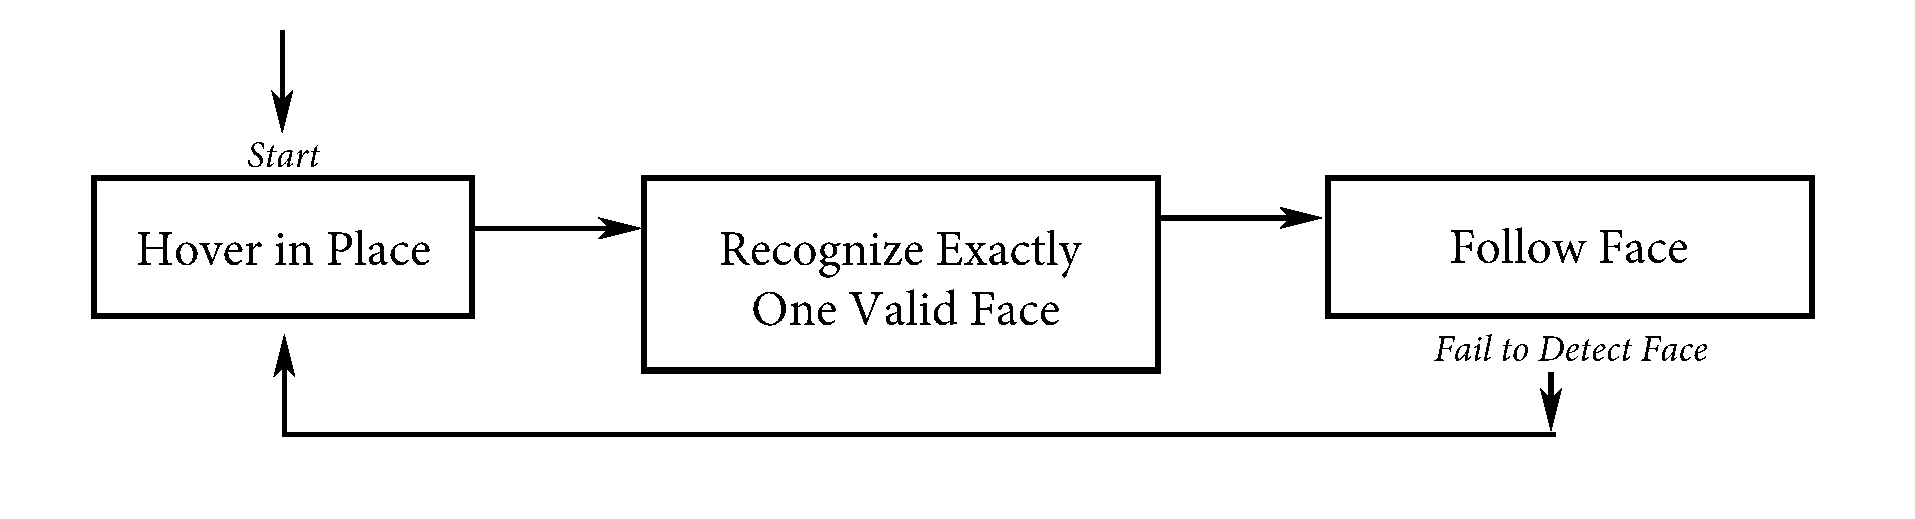
\includegraphics[width=6in]{quadrotor_state_diagram.pdf}
\end{figure}

Our live demonstration features untested computer vision algorithms to
pilot a possibly unstable flying robot to be developed in under three
weeks. Thus, we propose to bound the risk of a live demonstration by
first preparing foundational \textit{Base Flight} presentation which
we extend to prepare a second, more advanced \textit{Goal Flight}
presentation. The \textit{Base Presentation} is simple but sufficient,
and we complete and video record this Presentation by the second
week. Meanwhile, we individually prepare a cascade of more ambitious
sub-projects which more throughly fulfills the intended theoretical
computer vision emphasis of this class. Near the deadline, and we
compile the successful subprojects into an coherent \textit{Goal
  Flight} presentation as summarized above.

This split proposal grants us the flexibility to add, abandon, or
substitute subprojects without hindering core project progress or
risking a failure in the live demonstration, and it includes all group
members in substantial computer vision work. In the event of an
intractable complication, for example, total drone failure, we will
still be able to present a video demonstration of the flying drone
while striving to produce a more ambitious demonstration which we can
confidently and reasonably propose to complete by the project
deadline.

\section{Outline}
\begin{itemize}
\item \textbf{Project idea}: quadrotor object and face video tracker
\item \textbf{Data source}: streaming color 320x240 pixel video from
  embedded quadrotor video camera over local WiFi network connection
\item \textbf{Development and Code}: quadrotor video feed
  processing and pilot software in C++.
\item \textbf{Evaluation}: the quadrotor successfully follows the
  intended face or object.
\item \textbf{General Team Rolls}: 
  \begin{itemize}
  \item Michael: Video Analysis and Computer Vision
  \item Andrew: Project Management and Flight Control
  \item Daniya: Algorithms and Theory
  \end{itemize}
\end{itemize}


\section{Test Flight: Stationary Follow}

\textit{This flight is not intended to be a sufficient final
  presentation.\\\noindent To be completed by November 13th by Andrew.}\\

We propose to track and follow a green object while hovering above one
location for at least three minutes. To achieve this, the computer
vision techniques that we expect to use includes background
subtraction, simple threshold object detection and noise
filtering. The quadrotor will attempt to keep the green object in the
center of its view at a stable distance by rotating and lifting while
hovering in place. These algorithms will be written in C.

\subsection{Subgoal} Record sufficient corpus of training video to begin
independent work. This video may be recorded both with the drone
camera and with other cameras; for example, an iPhone video camera.

\begin{enumerate}
\item Detect single green object from video frame. Find centroid.
\item Compute (x,y) vector from object to center of frame.
\item Convert (x,y) vector to (rotate, lift) drone flight commands.
\item Follow green object until commanded to land from computer.
\end{enumerate}

\section{Base Flight: Dynamic Follow}
\textit{To be completed by November 20th by Andrew.}\\

We propose to track and follow one green ball in flight for at least
three minutes. The quadrotor will attempt to keep the green object in
the center of its view at a stable distance and will compensate for
the angular tilt and instability as the quadrotor pitches. To achieve
this, we extend the \textit{Test Flight} with computer vision
techniques including moment calculation, object scaling, and simple
object tracking. When the quadrotor does not detect the green ball, it
will hover in place. These algorithms will be written in C.

\begin{enumerate}
\item Select first green ball to enter video frame. Ignore all other
similar shapes (e.g. flat green frisbee)
\item Compute (x, y, z) vectors (z is distance to tracked object) from
  expected ball size. 
\item Convert (x,y,z) vector to rotate, lift, pitch flight commands
  given the current tilt of the drone.
\item Follow green ball until commanded to land from computer.
\end{enumerate}

\section{Subprojects}
\textit{To be completed by November 24th as listed
  individually. \\\noindent Individual project components may be
  programmed using C, C++, OpenCV, or Matlab.}

\subsection{Michael}
\begin{enumerate}
\item Skin Detection: select skin regions from color video frame

\item Face Detection: select face regions from set of candidate skin
regions. Determine approximate distance from drone to face.

\item Face Recognition: given a sufficiently large face-like object,
confirm that it is a face and recognize it as one of the three group
members.

\item End Face Detection: given a selected region that previously
  contained a face, detect when that face has been sufficiently
  obscured in order to halt tracking.
\end{enumerate}

\subsection{Daniya}
\begin{enumerate}
\item Object Track: Given a region, track that region frame to frame.
Compute this efficiently enough to be used in real time.

\item Tracked object trajectories: Given a selected object, compute the
smoothed motion trajectory of that object.

\item Matching trajectories: Given a smoothed trajectory, match that
trajectory to a model trajectory: shake up-down or shake left-right.
\end{enumerate}


\section{Goal Flight: Recognized Face Follow}
\textit{To be completed as a team by November 27th.}

We propose to integrate the work completed in the Subprojects into the
final ``Goal Flight'' demonstration as described in the Proposal
section. Subprojects that are incomplete or produce results too
unreliable to safely use in a live demonstration will be presented
using slides in a brief concluding presentation. We will also prepare
video recording of the goal flight which we may show if the drone
cannot be flown in class during the presentation due to, for example,
drone failure.

\begin{enumerate}
\item Hover in place.
\item Wait until exactly one identified face has been detected for at
  least three frames. If the drone detects any other faces in the
  scene, or if the face detected is not recognized as one of the group
  members, then continue to hover in place. 
\item Begin following the recognized face using object tracking. 
\item When tracked object is no longer detected as a face, stop
  following and hover in place.
\item Go back to 1.
\end{enumerate}



\end{spacing}
\end{document}

